\chapter{Testing chronosequence predictions with longitudinal data reveals microbial community convergence: Appendix S1}
%\chaptermark{Positive frequency-dependence}
%\renewcommand{\sectionmark}[1]{}
\fancyhead[LE, RO]{\thepage}
\fancyhead[RE]{APPENDIX D}
\fancyhead[LO]{TESTING CHRONOSEQUENCE WITH LONGITUDINAL DATA}
\fancyfoot{}
\renewcommand{\headrulewidth}{0pt}
\setlength{\parindent}{1cm}


\begin{comment}
\documentclass[hidelinks,12pt]{article}
\usepackage{graphicx,bm, booktabs,lineno,array}
\usepackage[fleqn]{amsmath}
\setlength{\mathindent}{0pt}
\usepackage[super,comma,numbers, compress]{natbib}
\usepackage[a4paper]{geometry}
\usepackage[parfill]{parskip}
\usepackage[usenames,dvipsnames]{color}
\usepackage[font=footnotesize,labelfont=bf,margin=1cm, labelsep = none]{caption} 
\usepackage{setspace}
\usepackage{gensymb}
\usepackage{color} 
\usepackage{sidecap}
\usepackage{epigraph}
\usepackage{float}
\usepackage{soul,xcolor}
\setstcolor{red}
\setlength\epigraphwidth{12cm}
\setlength\epigraphrule{0pt}
\usepackage{etoolbox}
\usepackage{tcolorbox}
\tcbuselibrary{breakable}
\usepackage[bottom, symbol]{footmisc}
\usepackage{authblk}
\usepackage{hyperref}
\usepackage[color=cyan]{todonotes}
\pdfminorversion=3
\doublespacing

\renewcommand{\epigraphflush}{center}
\renewcommand{\sourceflush}{flushleft}
\newcommand{\plus}{\raisebox{.4\height}{\scalebox{.6}{+}}}
\newcommand{\minus}{\raisebox{.4\height}{\scalebox{.8}{-}}}
\renewcommand{\thefootnote}{\fnsymbol{footnote}}
\newcommand*\samethanks[1][\value{footnote}]{\footnotemark[#1]}
\newcommand\blfootnote[1]{%
\begingroup
\renewcommand\thefootnote{}\footnote{#1}%
\addtocounter{footnote}{-1}%
\endgroup
}
\end{comment}



\begin{comment}
\begin{document}
	
\doublespacing
\title{Testing chronosequence predictions with longitudinal data reveals microbial community convergence}
\author[1, $\dagger$]{Po-Ju Ke}
\author[1, 2]{J. Nicholas Hendershot}
\author[1, $\dagger$]{Tadashi Fukami}
\affil[1]{Department of Biology, Stanford University, Stanford, California, USA}
\affil[2]{Center for Conservation Biology, Stanford University, Stanford, California, USA}
 
\date{\today}
\maketitle
\blfootnote{$\dagger$ Correspondence author: Department of Biology, Stanford University, Stanford, California 94305-5020, USA. Phone: +1 650-721-1711. Fax: +1 650-723-6132. Email: pojuke@stanford.edu, fukamit@stanford.edu}
	
\onehalfspacing
\noindent \textbf{Running title:} Predicting community structure with chronosequence\\
\noindent \textbf{Keywords:} beta diversity, \textit{Carpobrotus edulis}, community assembly, sand dunes, space-for-time substitution, succession\\
\noindent \textbf{Type of article:} Research article
	
\begin{myindentpar}{1cm}
	\textbf{Words in Abstract:} $\sim$ 200\\
	\textbf{Words in main text:} $\sim$ XXX\\
	\textbf{Number of references:} $\sim$ 50\\
	\textbf{Number of figures:} 5\\
\end{myindentpar}
	
\noindent \textbf{Authorship statement:} PJK and TF conceived the study; PJK conducted the study; PJK and JNH analyzed the data; PJK wrote the first draft of the manuscript with substantial contribution from all authors.\\
	
\noindent \textbf{Data accessibility statement:} Should the manuscript be accepted, all data and computer scripts supporting the results will be archived in a public repository, with the DOI included in the article.\\

\linenumbers
\doublespacing
\end{comment}



\section{Appendix S1 -- Supplementary Figures}
\clearpage
\begin{sidewaysfigure}[h]
	\centering
	\makebox[\textwidth][c]{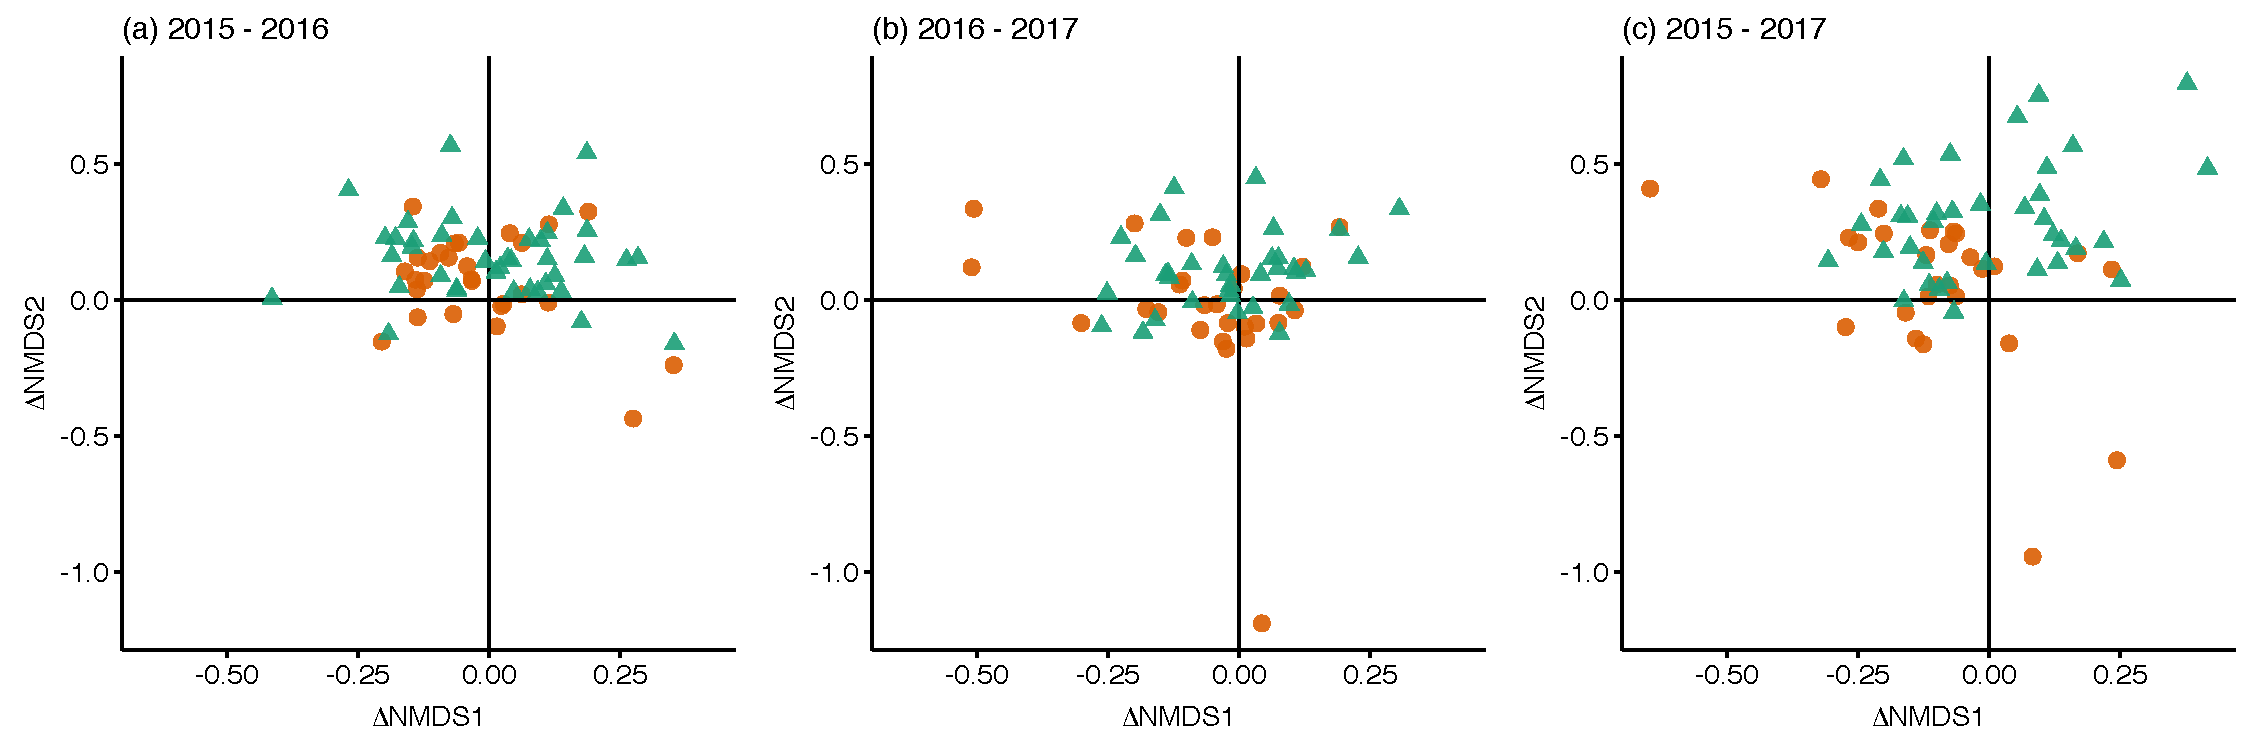
\includegraphics[width=18cm]{Chapter5/FourQuadrateMovement_Species_Common_RevisedSI.pdf}}
	\caption[Compositional shifts in fungal communities from the same plant individual among different sampling years.]
		{\hspace{1mm} Compositional shifts in fungal communities from the same plant individual among different sampling years. Each point represent the movement (i.e., x- and y-component of the arrow) on Fig.~\ref{fig:3YrNMDS_Individual}. A positive x-component (i.e., $\Delta$NMDS 1 $ > 0$) and y-component (i.e., $\Delta$NMDS 2 $ > 0$) represents a rightward and upward movement, respectively. (a) Shifts from 2015 to 2016; (b) shifts from 2016 to 2017; (c) shifts representing compositional differences between 2015 and 2017 (i.e., Fig.~\ref{fig:FourQuadrate_Individual_Species}). Point shapes and colors represent plant species (orange circle: \textit{C. edulis}; green triangle: \textit{L. arboreus}). 
		% See Fig.~\ref{fig:FourQuadrate_Sample_Species} for identical pattern when soil samples were plotted as observation units.
		}
	\label{fig:FourQuadrate_Individual_Species_SI}
\end{sidewaysfigure}



\clearpage
\begin{figure}[h]
	\centering
	\makebox[\textwidth][c]{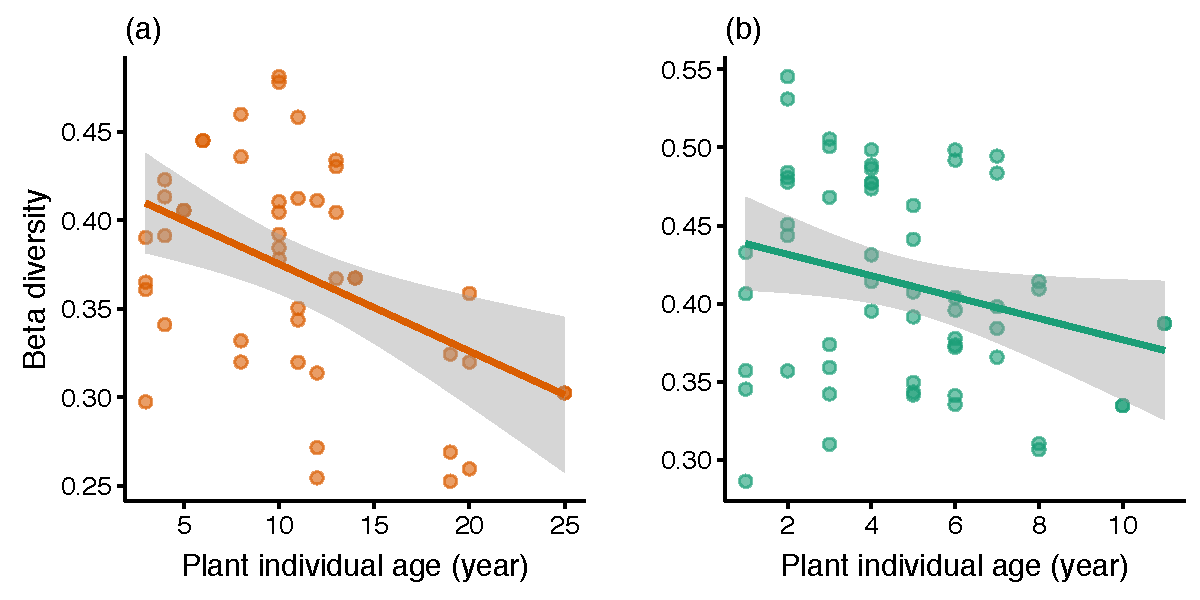
\includegraphics[width=15cm]{Chapter5/BetaDiversity_CompiledFull2015_Common_RevisedSI.pdf}}
	\caption[The relationship between plant age and beta diversity of fungal communities associated with chronosequence plant individuals.]
		{\hspace{1mm} The relationship between plant age and beta diversity of fungal communities associated with chronosequence plant individuals.
		(a) and (b) show the pattern for microbial communities associated with \textit{C. edulis} (orange) and \textit{L. arboreus} (green), respectively. 
		Each point represents the distance of one fungal community to the age-specific centroid.  
		% See Fig.~\ref{fig:Full2015Beta_Sample} for the pattern when soil samples were plotted as observation units.
		} 
	\label{fig:CombinedFull2015Beta_Individual_SI}
\end{figure}



\clearpage
\begin{figure}[h]
	\centering
	\makebox[\textwidth][c]{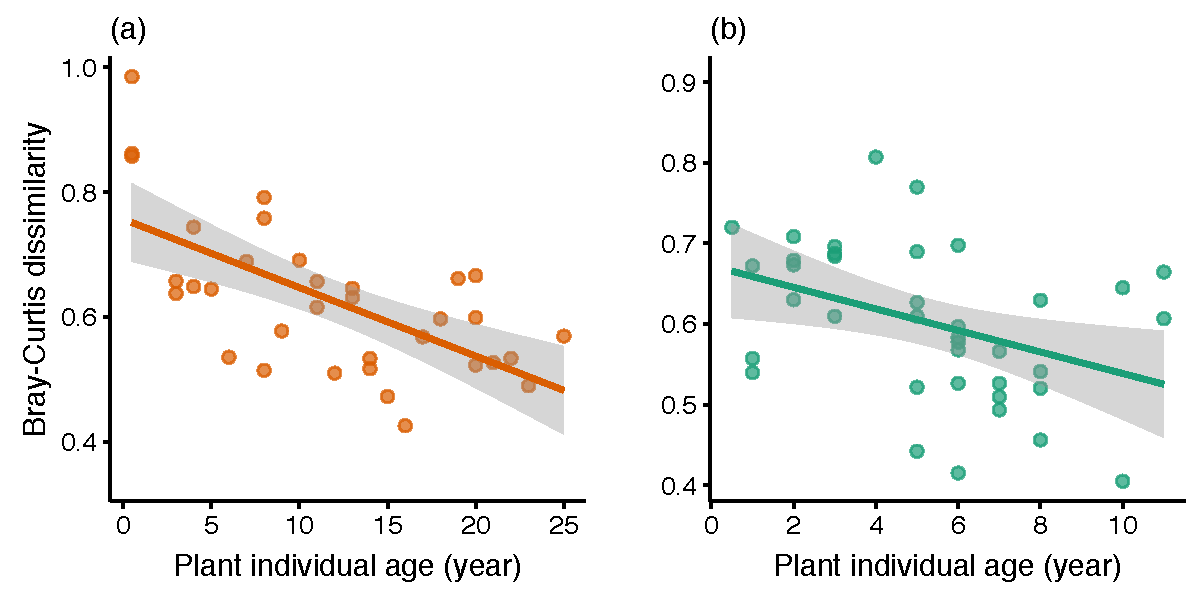
\includegraphics[width=15cm]{Chapter5/Goodness_FungiSpecies_CombinedIndividual_Full2015glmmTMBTotal_Revised2SI.pdf}}
	\caption[The relationship between plant age and Bray--Curtis dissimilarity between the fungal community observed in 2017 and the 2015 chronosequence prediction.]
		{\hspace{1mm} The relationship between plant age and Bray--Curtis dissimilarity between the fungal community observed in 2017 and the 2015 chronosequence prediction.
		(a) and (b) show the pattern for microbial communities associated with \textit{C. edulis} (orange) and \textit{L. arboreus} (green), respectively.
		Each point represents the dissimilarity calculated for a fungal community, using samples collected in 2017 as the validation test set. 
		% See Fig.~\ref{fig:HMSC_Species_Sample_Full2015} or identical pattern when soil samples were plotted as observation units.
		}
	\label{fig:HMSC_Species_Individual_Full2015_SI}
\end{figure}



\clearpage
\begin{figure}[h]
	\vspace*{-1cm}
	\centering
	\makebox[\textwidth][c]{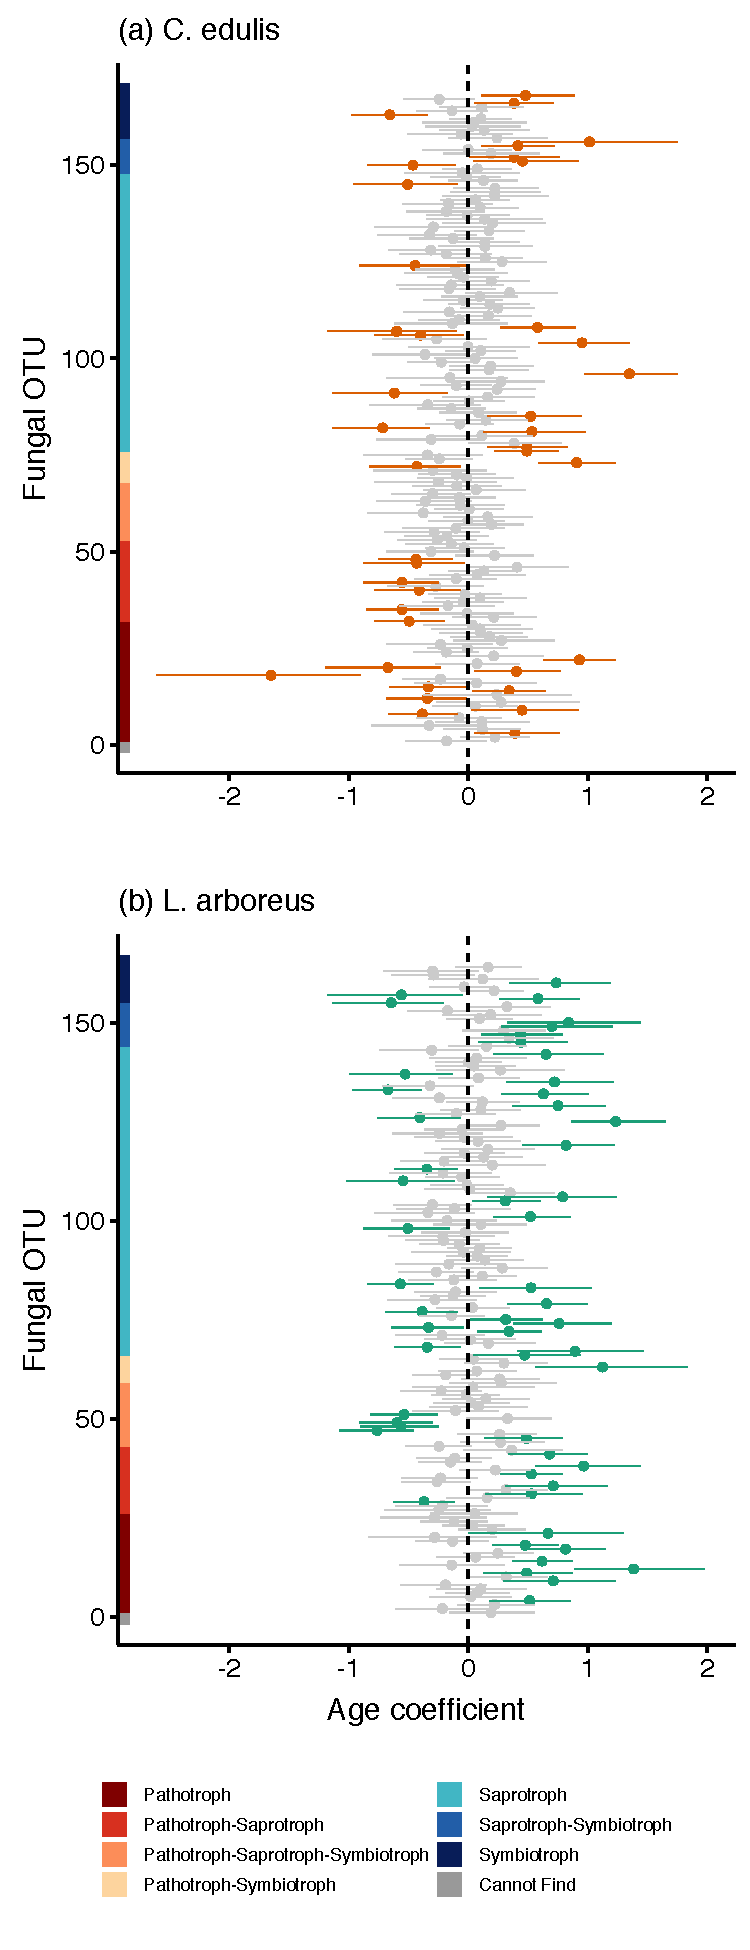
\includegraphics[width=7cm]{Chapter5/Funguild_HMSC_FungiSpecies_CombinedIndividual_Full2015Total_Long.pdf}}
	\caption[Predicted temporal trends and potential functional guilds of fungal OTUs associated with \textit{C. edulis} and \textit{L. arboreus}.]
		{\hspace{1mm} Predicted temporal trends and potential functional guilds of fungal OTUs associated with (a) \textit{C. edulis} and (b) \textit{L. arboreus}. Model fitting was performed for the two plant species separately. Points and line segments represent the mean and the 95$\%$ credible interval of the fitted age coefficient (x-axis) for different fungal OTUs (y-axis). Significant age coefficients are colored (orange for \textit{C. edulis}; green for \textit{L. arboreus}) and insignificant ones are in gray. Color codes along the y-axis are the predicted functional guild of the OTU obtained from \textit{FunGuild}.}
	\label{fig:Funguild_HMSC_Species_Individual_Full2015}
\end{figure}

